%Start
%required packages and reason
\documentclass[11pt]{article}
\usepackage[a4paper,margin=1in]{geometry}
\usepackage{mathtools} % required for sigma notation
\usepackage{graphicx} %required to load images
\usepackage{amsmath} %required for the matrices
\usepackage{upgreek} %required for Greek symbols
\usepackage{xfrac} %for differentiation symbol
\usepackage{float} %to set the figures exactly where we want,(\figure "[H]")
\usepackage{listings} %to get colorful code in latex
\usepackage{color} %to get a nice color scheme
\usepackage{pythonhighlight} %to make the the python codes nice

%initial headings
\title{EE2703 Assignment 9: Spectra of Non-Periodic Signals}
\author{Anvith Pabba [EE19B070]}
\date{30th May 2021}

%begin document
\begin{document}

\maketitle

\section{Abstract}
The goal of this Assignment is to:
\begin{enumerate}
    \item Find the Spectra of various non-periodic functions using numpy.fft.fft() and fftshift().
    \item Using window functions (in this case, Hammings Window) to obtain a more accurate DFT.
    \item Plotting and analysing the relevant graphs.
\end{enumerate}

\section{Introduction}
In the previous assignment we found the DFTs of periodic signals using the numpy.fft.fft() command and it gave us very accurate results. In this assignment we see the limitations of numpy.fft.fft() in finding the DFT of non-periodic signals and we understand how we can utilize \textbf{Windowing functions} in order to get accurate DFTs.\\~\\
Initially, we take a look at the Spectra of $sin(\sqrt{2}t)$ considering 64 samples over a range of $-\pi$ to $\pi$.

\begin{figure}[H]
    \centering
    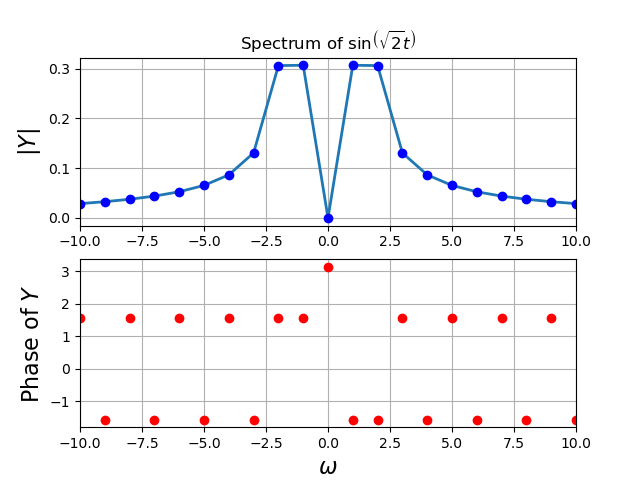
\includegraphics[scale = 0.75]{Figure_1.png}
    \caption{Spectra of $sin(\sqrt{2}t)$ with 64 samples}
\end{figure}

\subsection{Analysing the output Spectrum}
\begin{itemize}
    \item We can clearly see that there are \textbf{4} peaks when there should only be \textbf{2} peaks at $\omega=\sqrt{2}$.
    \item We see that the phase plot also follows a similar trend.
    \item The reason for this is because the DFT only works for functions that have a time period of $2\pi$. Which $sin(\sqrt{2}t)$ does not follow.
    \item We can see the non-periodic nature of $sin(\sqrt{2}t)$ in the following \textbf{Figure 2}
\end{itemize}

\subsection{Non-periodic nature of $sin(\sqrt{2}t)$}
\begin{figure}[H]
    \centering
    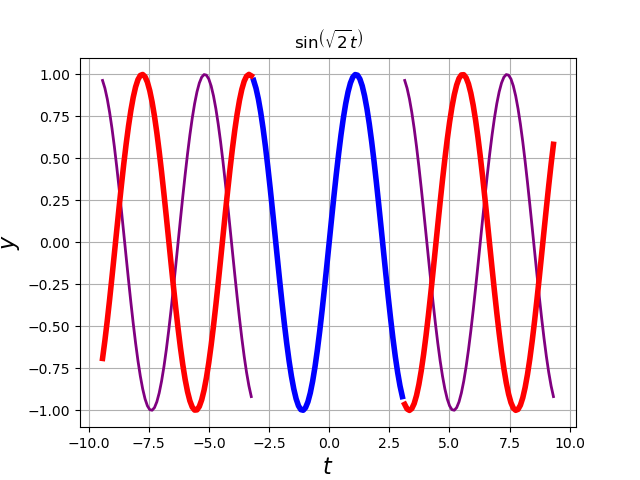
\includegraphics[scale = 0.75]{Figure_2.png}
    \caption{Non-periodic nature of $sin(\sqrt{2}t)$}
\end{figure}

\subsection{Analysing the above graph}
As we can clearly see, there are 3 colors of lines, these are:
\begin{enumerate}
    \item Blue: This is the plot of $sin(\sqrt{2}t)$ over a period of $-\pi$ to $\pi$.
    \item Red: This is actual remaining plot of $sin(\sqrt{2}t)$ vs time.
    \item Purple: This is the shifted plot of $sin(\sqrt{2}t)$ over a period of $-\pi$ to $\pi$ but it has been shifted for all the remaining $2\pi$ intervals as well.
\end{enumerate}
\begin{itemize}
    \item We can clearly see that the signal is not periodic with a periodic of $2\pi$.
    \item Infact, we can see that we are \textbf{Actually finding the DFT of the signal created by repeating the middle blue plot} (i.e the blue and purple plot).
    \item This is known as the \textbf{Periodic Extension of $sin(\sqrt{2}t)$ in the range of ($-\pi$,$\pi$)}.
\end{itemize}

\subsection{Code}
\begin{python}
#DFT of sin(sqrt(2)t)
t=linspace(-pi,pi,65);t=t[:-1]
dt=t[1]-t[0];fmax=1/dt
y=sin(sqrt(2)*t)
y[0]=0 # the sample corresponding to -tmax should be set zeroo
y=fftshift(y) # make y start with y(t=0)
Y=fftshift(fft(y))/64.0
w=linspace(-pi*fmax,pi*fmax,65);w=w[:-1]

subplot(2,1,1)
plot(w,abs(Y),w,abs(Y),'bo',lw=2)
xlim([-10,10])
ylabel(r"$|Y|$",size=16)
title(r"Spectrum of $\sin\left(\sqrt{2}t\right)$")
grid(True)

subplot(2,1,2)
plot(w,angle(Y),'ro',lw=2)
xlim([-10,10])
ylabel(r"Phase of $Y$",size=16)
xlabel(r"$\omega$",size=16)
grid(True)
show()


#plots of sin(sqrt(2)t) for different time ranges
t1=linspace(-pi,pi,65);t1=t1[:-1]
t2=linspace(-3*pi,-pi,65);t2=t2[:-1]
t3=linspace(pi,3*pi,65);t3=t3[:-1]

# y=sin(sqrt(2)*t)
plot(t1,sin(sqrt(2)*t1),'b',lw=4)
plot(t1+2*pi,sin(sqrt(2)*t1),'purple',lw=2)
plot(t1-2*pi,sin(sqrt(2)*t1),'purple',lw=2)
plot(t2,sin(sqrt(2)*t2),'r',lw=4)
plot(t3,sin(sqrt(2)*t3),'r',lw=4)
ylabel(r"$y$",size=16)
xlabel(r"$t$",size=16)
title(r"$\sin\left(\sqrt{2}t\right)$")
grid(True)
show()
\end{python}

\section{Windowing Function: The Hamming Window}
We can clearly see in Figure 2 that at the ends of the periodic interval, for example at the end of $\pi$, there are huge discontinuities. This is the reason our DFT results are not as accurate as we expect.\\~\\
In order to fix this, we damp the function near there, i.e, we multiply our function sequence f [n] by a “window” sequence w[n]:
\begin{equation}
    g(n)=f(n)w(n)
\end{equation}
We get the new spectrum by convolving the two Fourier transforms.
\begin{equation}
    G_k=\sum_{n=0}^{N-1}F_nW_{k-n}
\end{equation}
The window we use is called the Hamming window, which is given by:
\[   
w[n] = 
    \begin{cases}
        \text{0.54+0.46cos($\frac{2\pi n}{N-1}$)} &\quad\text{$|n|<$N} \\ 
        \text{0} &\quad\text{else} \\ 
    \end{cases}
\]

\subsection{Plot of $sin(\sqrt{2}t)$ after multiplying with the Hamming Window}
\begin{figure}[H]
    \centering
    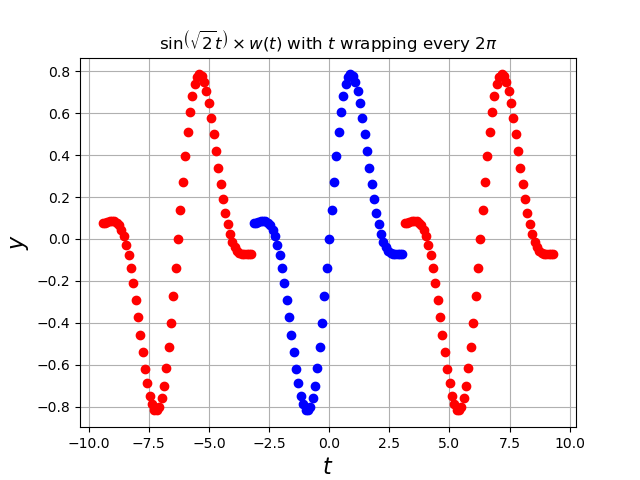
\includegraphics[scale = 0.75]{Figure_3.png}
    \caption{Plot of $sin(\sqrt{2}t)$ after Windowing}
\end{figure}

\subsection{Code for the above}
\begin{python}
#plot of sin(sqrt(2)t) after windowing:
t1=linspace(-pi,pi,65);t1=t1[:-1]
t2=linspace(-3*pi,-pi,65);t2=t2[:-1]
t3=linspace(pi,3*pi,65);t3=t3[:-1]
n=arange(64)
wnd=fftshift(0.54+0.46*cos(2*pi*n/63))
y=sin(sqrt(2)*t1)*wnd
figure(3)
plot(t1,y,'bo',lw=2)
plot(t2,y,'ro',lw=2)
plot(t3,y,'ro',lw=2)
ylabel(r"$y$",size=16)
xlabel(r"$t$",size=16)
title(r"$\sin\left(\sqrt{2}t\right)\times w(t)$ with $t$ wrapping every $2\pi$ ")
grid(True)
show()
\end{python}

\subsection{DFT of the signal after Windowing}
\subsubsection{Spectrum of the signal only taking 64 points}
\begin{figure}[H]
    \centering
    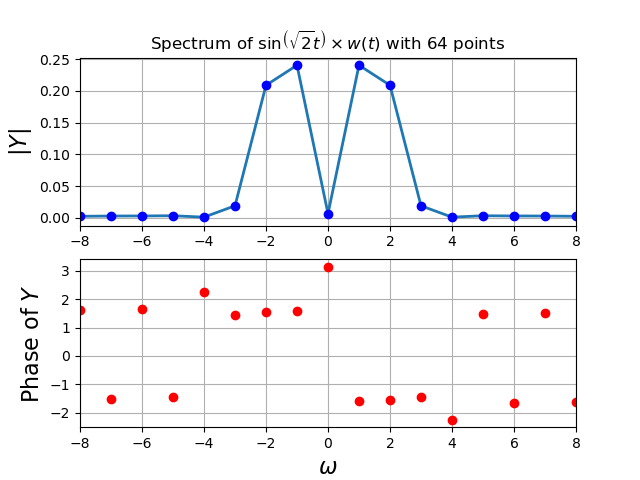
\includegraphics[scale = 0.75]{Figure_4.png}
    \caption{DFT of $sin(\sqrt{2}t)$ after Windowing with 64 points}
\end{figure}

We now find the Spectrum after increasing the number of samples taken to 256.

\subsubsection{Spectrum of the signal only taking 256 points}
\begin{figure}[H]
    \centering
    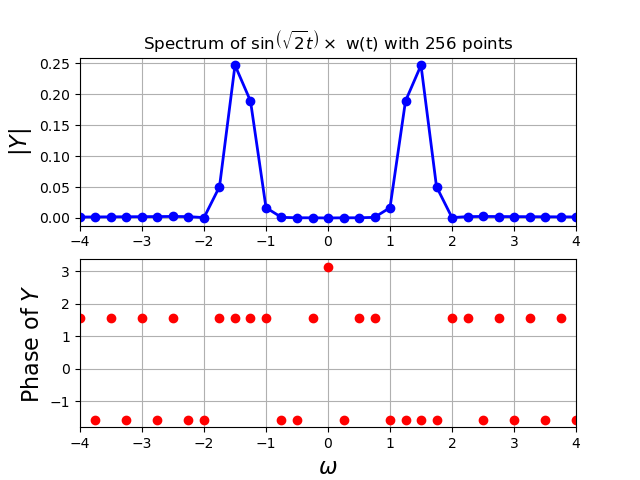
\includegraphics[scale = 0.75]{Figure_5.png}
    \caption{DFT of $sin(\sqrt{2}t)$ after Windowing with 256 points}
\end{figure}
We can clearly see that the Spectrum has become more accurate.

\subsection{Code}
\begin{python}
#DFT of the function after windowing

t=linspace(-pi,pi,65);t=t[:-1]
dt=t[1]-t[0];fmax=1/dt
n=arange(64)
wnd=fftshift(0.54+0.46*cos(2*pi*n/63))
y=sin(sqrt(2)*t)*wnd
y[0]=0 # the sample corresponding to -tmax should be set zeroo
y=fftshift(y) # make y start with y(t=0)
Y=fftshift(fft(y))/64.0
w=linspace(-pi*fmax,pi*fmax,65);w=w[:-1]

subplot(2,1,1)
plot(w,abs(Y),w,abs(Y),'bo',lw=2)
xlim([-8,8])
ylabel(r"$|Y|$",size=16)
title(r"Spectrum of $\sin\left(\sqrt{2}t\right)\times w(t)$ with 64 points")
grid(True)

subplot(2,1,2)
plot(w,angle(Y),'ro',lw=2)
xlim([-8,8])
ylabel(r"Phase of $Y$",size=16)
xlabel(r"$\omega$",size=16)
grid(True)
show()

#DFT after windowing with 256 points


t=linspace(-4*pi,4*pi,257);t=t[:-1]
dt=t[1]-t[0];fmax=1/dt
n=arange(256)
wnd=fftshift(0.54+0.46*cos(2*pi*n/256))
y=sin(sqrt(2)*t)
# y=sin(1.25*t)
y=y*wnd
y[0]=0 # the sample corresponding to -tmax should be set zeroo
y=fftshift(y) # make y start with y(t=0)
Y=fftshift(fft(y))/256.0
w=linspace(-pi*fmax,pi*fmax,257);w=w[:-1]

subplot(2,1,1)
plot(w,abs(Y),'b',w,abs(Y),'bo',lw=2)
xlim([-4,4])
ylabel(r"$|Y|$",size=16)
title(r"Spectrum of $\sin\left(\sqrt{2}t\right)\times$ w(t) with 256 points")
grid(True)

subplot(2,1,2)
plot(w,angle(Y),'ro',lw=2)
xlim([-4,4])
ylabel(r"Phase of $Y$",size=16)
xlabel(r"$\omega$",size=16)
grid(True)
show()
\end{python}



\section{Q2: Spectrum of $cos^3(0.86t$ before and after windowing}
We plot the spectrum's in the figures below:

\subsection{Spectrum of $cos^3(0.86t$ before Windowing}
\begin{figure}[H]
    \centering
    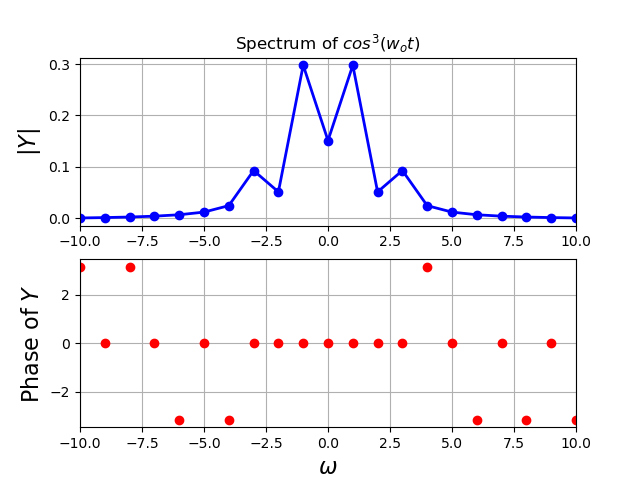
\includegraphics[scale = 0.75]{Figure_6.png}
    \caption{Spectrum of $cos^3(0.86t$ before Windowing}
\end{figure}

\subsection{Spectrum of $cos^3(0.86t$ after Windowing}
\begin{figure}[H]
    \centering
    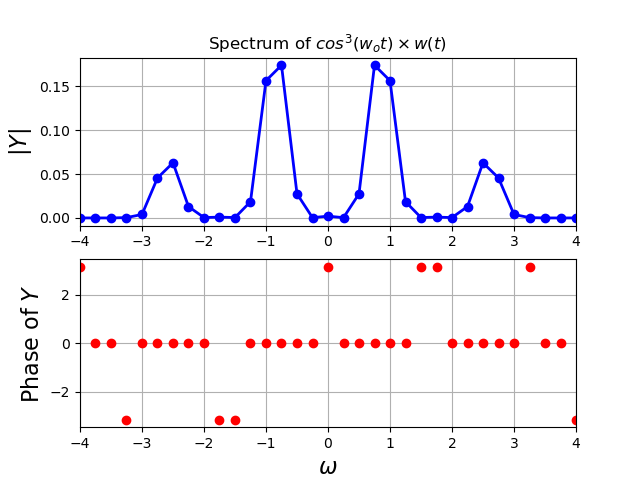
\includegraphics[scale = 0.75]{Figure_7.png}
    \caption{Spectrum of $cos^3(0.86t$ after Windowing}
\end{figure}

\subsection{Code}
\begin{python}
#Question 2:

#DFT of cos^3(wot) where wo=0.86 without hamming window

t=linspace(-pi,pi,257);t=t[:-1]
dt=t[1]-t[0];fmax=1/dt
wo=0.86
y=(cos(wo*t))**3
y[0]=0 # the sample corresponding to -tmax should be set zeroo
y=fftshift(y) # make y start with y(t=0)
Y=fftshift(fft(y))/256.0
w=linspace(-pi*fmax,pi*fmax,257);w=w[:-1]

subplot(2,1,1)
plot(w,abs(Y),'b',w,abs(Y),'bo',lw=2)
xlim([-10,10])
ylabel(r"$|Y|$",size=16)
title(r"Spectrum of $cos^3(w_ot)$")
grid(True)


subplot(2,1,2)
plot(w,angle(Y),'ro',lw=2)
xlim([-10,10])
ylabel(r"Phase of $Y$",size=16)
xlabel(r"$\omega$",size=16)
grid(True)
show()



#DFT of cos^3(wot) where wo=0.86 with the hamming window


t=linspace(-4*pi,4*pi,257);t=t[:-1]
dt=t[1]-t[0];fmax=1/dt
n=arange(256)
wnd=fftshift(0.54+0.46*cos(2*pi*n/256))
wo=0.86
y=(cos(wo*t))**3
# y=cos^3(wo*t)
y=y*wnd
y[0]=0 # the sample corresponding to -tmax should be set zeroo
y=fftshift(y) # make y start with y(t=0)
Y=fftshift(fft(y))/256.0
w=linspace(-pi*fmax,pi*fmax,257);w=w[:-1]


subplot(2,1,1)
plot(w,abs(Y),'b',w,abs(Y),'bo',lw=2)
xlim([-4,4])
ylabel(r"$|Y|$",size=16)
title(r"Spectrum of $cos^3(w_ot)\times w(t)$")
grid(True)


subplot(2,1,2)
plot(w,angle(Y),'ro',lw=2)
xlim([-4,4])
ylabel(r"Phase of $Y$",size=16)
xlabel(r"$\omega$",size=16)
grid(True)
show()
\end{python}


\section{Q3: Estimating the $\omega _o$ and $\delta$ of a $cos(\omega _ot+\delta)$ signal}
\begin{itemize}
    \item In this part of the code, we have a function that \textbf{Randomly generates a $\omega _o$ and a $\delta$} and plots the DFT of the randomly obtained function.
    \item \textbf{NOTE: the values of $\omega _o$ and $\delta$ change every time you run the code as they are RANDOMLY GENERATED}
    \item According to the conditions given in the Question, the resolution of the code will not be clear enough that we can directly find the peaks and call that $\omega _o$, instead, we have to extract all the information we can from the graoh to get these values.
    \item Hence, we find the \textbf{Weighted mean} of all the points with magnitude greater than 0.
    \item the Equation is as follows:
    \begin{equation}
        \omega _o= \frac{\Sigma \omega _k|Y(\omega _k)|^2}{\Sigma |Y(\omega _k)|^2} \;\; \forall\:w _k>0
    \end{equation}
    \item To estimate $\delta$, we just find the phase of the DFT at the points close to the point of maximum amplitude.
    \item This approach is based on the fact that for $\delta=0$, the phase of the maximum point is 0. But for a non-zero $\delta$, the $\delta$ we obtain is the required $\delta$.
    \item We multiply it with the Hamming window to get accurate results.
\end{itemize}

\subsection{Outputs}
The outputs one gets is:
\begin{enumerate}
    \item A line telling them the actual $\omega _o$ and $\delta$.
    \item A line telling them the estimated $\omega _o$.
    \item A line telling them the estimated $\delta$.
    \item Spectrum plots of the function
\end{enumerate}

\subsection{An Example plot}
\begin{figure}[H]
    \centering
    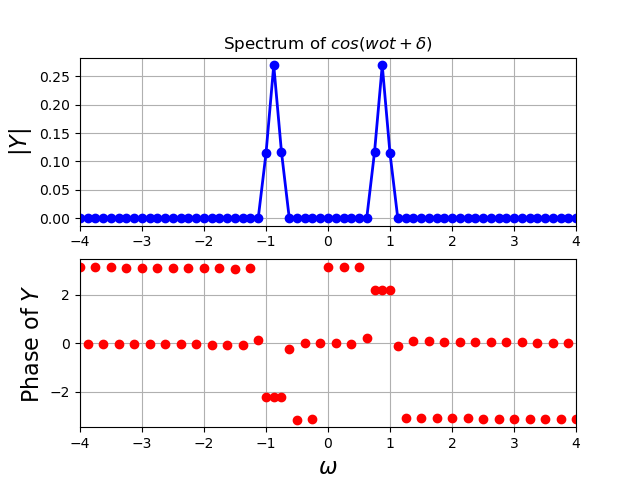
\includegraphics[scale = 0.75]{Figure_8.png}
    \caption{Spectrum of cos($\omega _o$t + $\delta$)}
\end{figure}

\subsection{Terminal Output}
\begin{figure}[H]
    \centering
    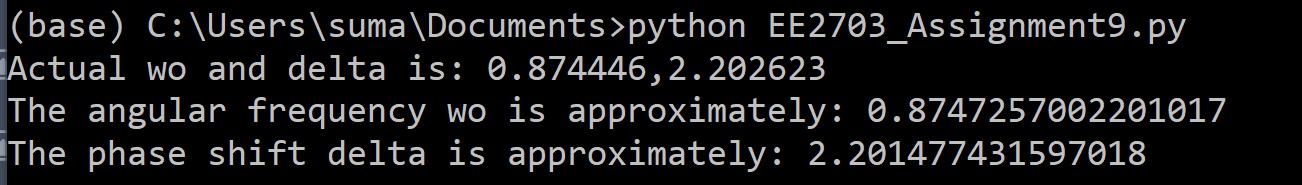
\includegraphics[scale = 0.75]{Output_1.jpg}
    \caption{Output of terminal}
\end{figure}
As we can clearly see, 
\begin{enumerate}
    \item the actual randomly generated $\omega _o$ is 0.874446 
    \item the actual randomly generated $\delta$ is 2.202623
\end{enumerate}
The estimated $\omega _o$ and $\delta$ are:
\begin{enumerate}
    \item estimated $\omega _o$ = 0.8747257002201017
    \item estimated $\omega _o$ = 2.201477431597018
\end{enumerate}
\textbf{SUCCESS!!, We can clearly see that the estimated value are very very similar to the actual randomly generated values.}

\section{Q4: Estimating the $\omega _o$ and $\delta$ of a $cos(\omega _ot+\delta)$ \textbf{Noisy} signal}
We add a gaussian white noise of amplitude 0.1 to make the signal noisy.\\~\\
\textbf{AGAIN NOTE, the values of $\omega _o$ and $\delta$ change every time you run the code as they are RANDOMLY GENERATED}.\\~\\
The process for estimated the values here is extremely similar to the process we used in the previous question, but here we need to take the weighted mean of signals with magnitude greater than 0.15. i.e,
\begin{equation}
    \omega _o= \frac{\Sigma \omega _k|Y(\omega _k)|^{1.6}}{\Sigma |Y(\omega _k)|^{1.6}} \;\; \forall\:w _k>0.15
\end{equation}
This power of 1.6 was obtained through trial and error until I got the lowest error between actual and estimated values of the variables for HIGHEST number of cases.

\subsection{Outputs}
The outputs one gets is:
\begin{enumerate}
    \item A line telling them the actual $\omega _o$ and $\delta$.
    \item A line telling them the estimated noisy $\omega _o$.
    \item A line telling them the estimated noisy $\delta$.
    \item Spectrum plots of the noisy function
\end{enumerate}

\subsection{An Example noisy plot}
\begin{figure}[H]
    \centering
    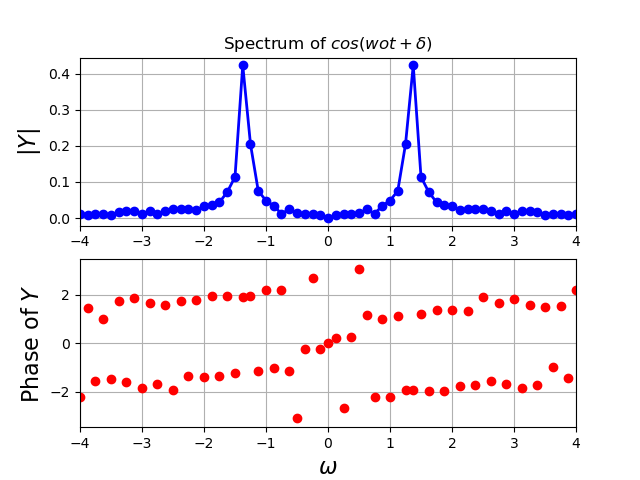
\includegraphics[scale = 0.75]{Figure_9.png}
    \caption{Spectrum of noisy cos($\omega _o$t + $\delta$)}
\end{figure}

\subsection{Terminal Output}
\begin{figure}[H]
    \centering
    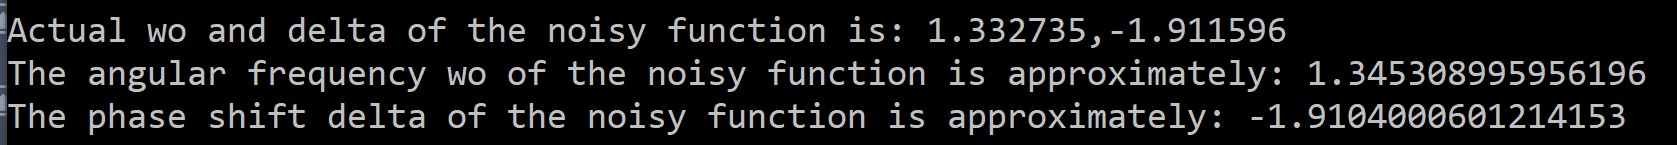
\includegraphics[scale = 0.75]{Output_2.jpg}
    \caption{Output of terminal}
\end{figure}
As we can clearly see, 
\begin{enumerate}
    \item the actual randomly generated noisy $\omega _o$ is 1.332735
    \item the actual randomly generated noisy $\delta$ is -1.911596
\end{enumerate}
The estimated $\omega _o$ and $\delta$ are:
\begin{enumerate}
    \item estimated noisy $\omega _o$ = 1.345308995956196
    \item estimated noisy $\omega _o$ = -1.9104000601214153
\end{enumerate}
\textbf{SUCCESS!!, We can clearly see that the estimated value are very very similar to the actual randomly generated values.}

\subsection{Code for Q3}
\begin{python}
#Question 3: finding wo and delta from a randomly generated vector

N=128

wo = random() + 0.5
delta = random()*2*pi - pi
t=linspace(-8*pi,8*pi,N+1);t=t[:-1] #time period of -pi to pi has very low precision
dt = t[1]-t[0];fmax=1/dt
n = arange(N)
wnd = fftshift(0.54+0.46*cos(2*pi*n/N))
vec = cos(wo*t + delta)
vec = vec*wnd
vec[0]=0 # the sample corresponding to -tmax should be set zeroo
y=fftshift(vec) # make y start with y(t=0)
Y=fftshift(fft(y))/N
w=linspace(-pi*fmax,pi*fmax,N+1);w=w[:-1]
print('Actual wo and delta is: %f,%f'%(wo,delta))

subplot(2,1,1)
plot(w,abs(Y),'b',w,abs(Y),'bo',lw=2)
ylabel(r"$|Y|$",size=16)
xlim([-4,4])
title(r"Spectrum of $cos(wot+\delta)$")
grid(True)

subplot(2,1,2)
plot(w,angle(Y),'ro',lw=2)
ylabel(r"Phase of $Y$",size=16)
xlabel(r"$\omega$",size=16)
xlim([-4,4])
grid(True)
show()

max = abs(Y).max()
ii = where(abs(abs(Y)-(max))<0.01)
ii2 = where(abs(Y)>0)
wapprox = sum(abs(Y[ii2])*abs(Y[ii2])*abs(w[ii2])) / sum(abs(Y[ii2])*abs(Y[ii2]))
print('The angular frequency wo is approximately:',wapprox)
print('The phase shift delta is approximately:',angle(Y[ii][1]))
\end{python}

\subsection{Code for Q4}
\begin{python}
#Question 4: Same as above, but now we find it for a noisy signal

N=256

wo = random() + 0.5
delta = random()*2*pi - pi
t=linspace(-8*pi,8*pi,N+1);t=t[:-1] #time period of -pi to pi has very low precision
dt = t[1]-t[0];fmax=1/dt
vec = cos(wo*t + delta)
vec = vec + 0.1*randn(N)
vec[0]=0 # the sample corresponding to -tmax should be set zeroo
y=fftshift(vec) # make y start with y(t=0)
Y=fftshift(fft(y))/N
w=linspace(-pi*fmax,pi*fmax,N+1);w=w[:-1]
print('\nActual wo and delta of the noisy function is: %f,%f'%(wo,delta))

subplot(2,1,1)
plot(w,abs(Y),'b',w,abs(Y),'bo',lw=2)
xlim([-4,4])
ylabel(r"$|Y|$",size=16)
title(r"Spectrum of $cos(wot+\delta)$")
grid(True)


subplot(2,1,2)
plot(w,angle(Y),'ro',lw=2)
xlim([-4,4])
ylabel(r"Phase of $Y$",size=16)
xlabel(r"$\omega$",size=16)
grid(True)
show()

max = abs(Y).max()
ii = where(abs(abs(Y)-(max))<0.01)
ii2 = where(abs(Y)>0.15)
wapprox = sum(abs(Y[ii2])**1.6*abs(w[ii2])) / sum(abs(Y[ii2])**1.6)
print('The angular frequency wo of the noisy function is approximately:',wapprox)
print('The phase shift delta of the noisy function is approximately:',angle(Y[ii][1]))
\end{python}

\section{Q5: Spectrum of the Chirped Signal}
The \textbf{Chirped signal} is given by:
\begin{equation}
    y(t)=cos(16(1.5+\frac{t}{2\pi})t)
\end{equation}
its frequency continuously changes from 16 radians per second near $-\pi$ to 32 radians per second near $\pi$.

\subsection{Spectrum of the Chirped Signal without hamming window}
\begin{figure}[H]
    \centering
    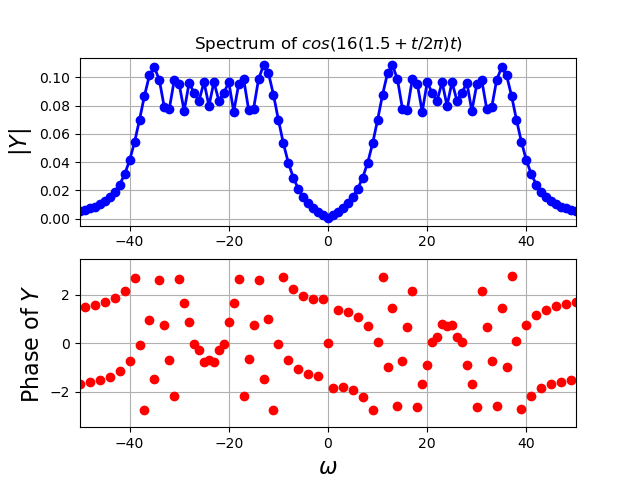
\includegraphics[scale = 0.75]{Figure_10.png}
    \caption{Spectrum of the Chirped Signal without hamming window}
\end{figure}

\subsection{Spectrum of the Chirped Signal with hamming window}
\begin{figure}[H]
    \centering
    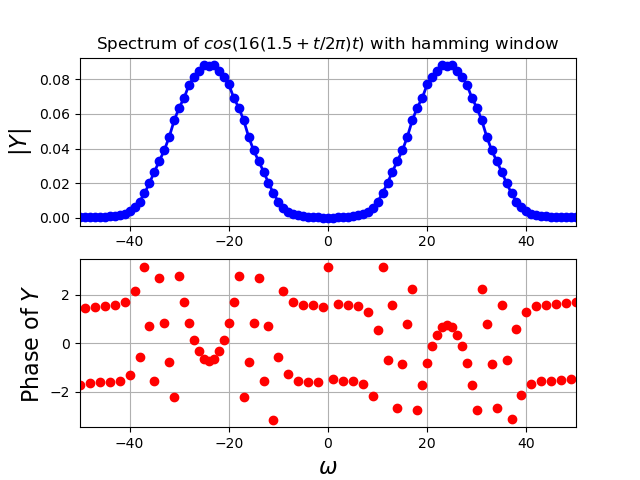
\includegraphics[scale = 0.75]{Figure_10b.png}
    \caption{Spectrum of the Chirped Signal with hamming window}
\end{figure}

\subsection{Code}
\begin{python}
#Question 5: DFT of a 'chirped' signal

N=1024

t=linspace(-pi,pi,N+1);t=t[:-1] #time period of -pi to pi has very low precision
dt = t[1]-t[0];fmax=1/dt
y = cos(16*t*(1.5 + (t/(2*pi))))
y[0]=0 # the sample corresponding to -tmax should be set zeroo
y=fftshift(y) # make y start with y(t=0)
Y=fftshift(fft(y))/N
w=linspace(-pi*fmax,pi*fmax,N+1);w=w[:-1]

subplot(2,1,1)
plot(w,abs(Y),'b',w,abs(Y),'bo',lw=2)
xlim([-50,50])
ylabel(r"$|Y|$",size=16)
title(r"Spectrum of $cos(16(1.5+t/2\pi)t)$")
grid(True)


subplot(2,1,2)
plot(w,angle(Y),'ro',lw=2)
xlim([-50,50])
ylabel(r"Phase of $Y$",size=16)
xlabel(r"$\omega$",size=16)
grid(True)
show()

#with hamming window
N=1024

t=linspace(-pi,pi,N+1);t=t[:-1] #time period of -pi to pi has very low precision
dt = t[1]-t[0];fmax=1/dt
n = arange(N)
wnd = fftshift(0.54+0.46*cos(2*pi*n/N))
y = cos(16*t*(1.5 + (t/(2*pi))))
y = y*wnd
y[0]=0 # the sample corresponding to -tmax should be set zeroo
y=fftshift(y) # make y start with y(t=0)
Y=fftshift(fft(y))/N
w=linspace(-pi*fmax,pi*fmax,N+1);w=w[:-1]

subplot(2,1,1)
plot(w,abs(Y),'b',w,abs(Y),'bo',lw=2)
xlim([-50,50])
ylabel(r"$|Y|$",size=16)
title(r"Spectrum of $cos(16(1.5+t/2\pi)t)$ with hamming window")
grid(True)


subplot(2,1,2)
plot(w,angle(Y),'ro',lw=2)
xlim([-50,50])
ylabel(r"Phase of $Y$",size=16)
xlabel(r"$\omega$",size=16)
grid(True)
show()
\end{python}

\section{Q6: Surface Plot of Variation of frequency with time - Chirped Signal}
We now use a surface plot to visualise how the frequency of the signal varies with time.
\begin{enumerate}
    \item We first break the 1024 vector into pieces that are 64 samples wide.
    \item We then Extract the DFT of each and store as a column in a 2D array (variable name is 'subvec'.)
    \item Unfortunately, we need to use atleast 1 for loop to execute what we want.
    \item Finally, plot the array as a surface plot to show how the frequency of the signal varies with time.
\end{enumerate}
The surface plots for the chirped signal are given in the plots below:

\subsection{Surface Plot of Variation of frequency with time - Chirped Signal without Windowing}
\begin{figure}[H]
    \centering
    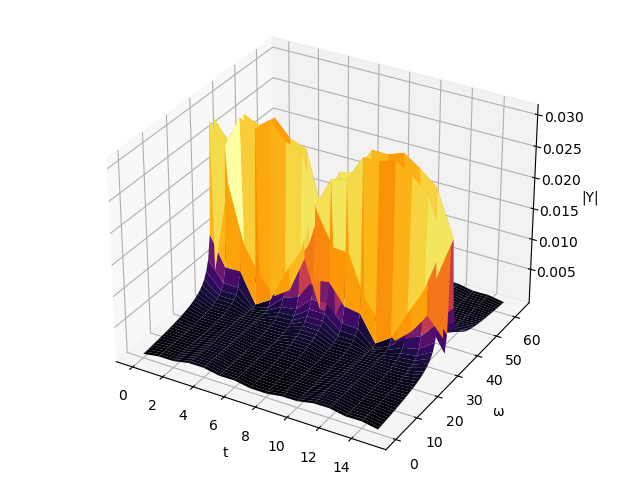
\includegraphics[scale = 0.75]{Figure_11.png}
    \caption{Surface Plot of Variation of frequency with time - Chirped Signal without Windowing}
\end{figure}

\subsection{Surface Plot of Variation of frequency with time - Chirped Signal with Windowing}
\begin{figure}[H]
    \centering
    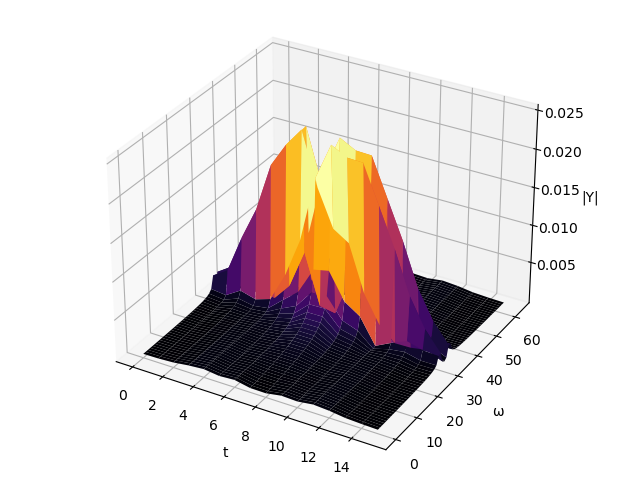
\includegraphics[scale = 0.75]{Figure_12.png}
    \caption{Surface Plot of Variation of frequency with time - Chirped Signal with Windowing}
\end{figure}

\subsection{Code for without windowing}
\begin{python}
#Question 6: Surface Plot of Variation of frequency with time for both types of chirped signals
#Without hamming window:

N=1024

t=linspace(-pi,pi,N+1);t=t[:-1] #time period of -pi to pi has very low precision
dt = t[1]-t[0];fmax=1/dt
y = cos(16*t*(1.5 + (t/(2*pi))))

subvec = zeros((16,64))
for n in arange(16):
    subvec[n]=y[64*n:64*n + 64]
    subvec[n][0] = 0

y=fftshift(subvec) # make y start with y(t=0)
Y=fftshift(fft(y))/N
w=linspace(-pi*fmax,pi*fmax,N+1);w=w[:-1]
n=arange(64)


t1 = np.array ( arange (16) )
t1,n = meshgrid ( t1 , n )
ax = Axes3D(figure())
surf = ax.plot_surface ( t1 ,n ,abs(Y).T , rstride =1 , cstride =1 , cmap ='inferno')
ylabel('\u03C9')
xlabel('t')
title(" Surface Plot of Variation of frequency with time - Chirped Signal without Hamming Window ")
ax.set_zlabel ('|Y|')
show()
\end{python}

\subsection{Code for with windowing}
\begin{python}
#With hamming window:
N=1024

t=linspace(-pi,pi,N+1);t=t[:-1] #time period of -pi to pi has very low precision
dt = t[1]-t[0];fmax=1/dt
n = arange(N)
wnd = fftshift(0.54+0.46*cos(2*pi*n/N))
y = cos(16*t*(1.5 + (t/(2*pi))))
y = y*wnd

subvec = zeros((16,64))
for n in arange(16):
    subvec[n]=y[64*n:64*n + 64]
    subvec[n][0] = 0


y=fftshift(subvec) # make y start with y(t=0)
Y=fftshift(fft(y))/N
w=linspace(-pi*fmax,pi*fmax,N+1);w=w[:-1]
n=arange(64)


t1 = np.array ( arange (16) )
t1,n = meshgrid ( t1 , n )
ax = Axes3D( figure())
surf = ax.plot_surface ( t1 ,n ,abs(Y).T , rstride =1 , cstride =1 , cmap ='inferno')
ylabel('\u03C9')
xlabel('t')
title(" Surface Plot of Variation of frequency with time - Chirped Signal with Hamming Window ")
ax.set_zlabel ('|Y|')
show()

#end
\end{python}












\end{document}